\documentclass[11pt,letterpaper]{article}
\usepackage{amssymb,amsmath,graphicx,url}
\pdfpagewidth=8.5truein
\pdfpageheight=11.0truein
\setlength{\topmargin}{-.5in}

\setlength{\textheight}{8.875in}
\setlength{\textwidth}{6.5in}
\setlength{\oddsidemargin}{-.1875in}  % Centers text.
\setlength{\evensidemargin}{-.1875in}
\usepackage{graphicx}
\begin{document}
\begin{center}
\section*{Homework 1: CSCI 6212 Algorithms, Fall 2019}    
\end{center}
\subsection*{Due: Beginning of class, September 20, 2019}

    \subsection*{Collaboration Policies:} This is not a group homework, you are required to do this homework yourself.  However, you are {\em allowed} to:
    \begin{itemize} 
    \item use or search any passive online resource for information about how to solve the problem.  
    \item discuss the problems with classmates.  
    \end{itemize}
    You are {\em not allowed} to
    \begin{itemize} 
    \item use active web resources (like Stack Overflow) where you post questions and ask for responses.
    \item post these questions to a "work for hire" site where someone else does them for you.
    \item take *any* written notes from discussions with classmates or others. 
    \end{itemize}

Please note, not all homeworks this semester will be this short, or this focused on multiple choice answers.  Good luck!

\begin{enumerate}
    \item Sort the following functions from asymptotically smallest to asymptotically largest, indicating ties if there are any. Do not submit proofs, just a sorted list of 16 functions.

    Write $f(n) \prec g(n)$ to indicate that $f(n) = o(g(n))$, and write $f(n) \equiv g(n)$ to mean $f(n) = \Theta(g(n))$.  We use the notation $lg(n)  = log_2(n)$.

\begin{center}    
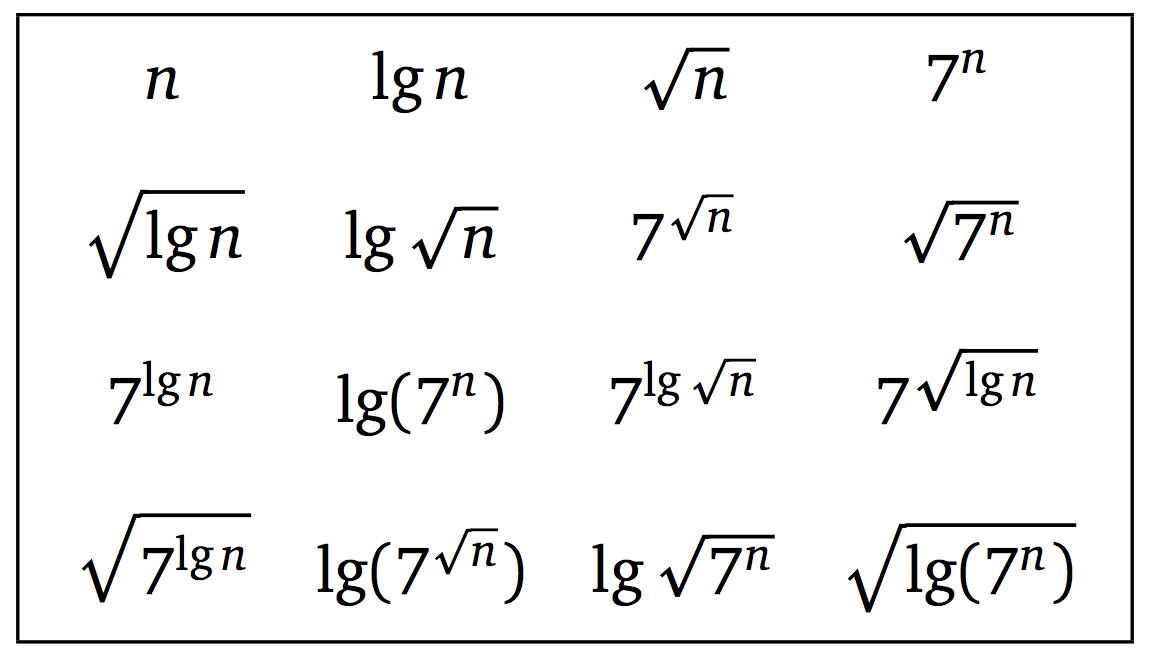
\includegraphics[width=3in]{figs/hw1_sevens.png}
\end{center}    
    A {\em wrong} answer, in the correct format, might look like:
    
    $$ n \prec lg~n \equiv 7^{\sqrt{n}} \equiv 7^{lg~\sqrt{n}} \prec\sqrt{lg~n} \ldots $$

\item The following are the time complexity for 4 different functions.  For each, solve the recurrence and give them complexity in $\Theta$ notation
\begin{enumerate}
    \item $T(n) = 3T(\frac{n}{3}) + 1$
    \item $T(n) = 3T(\frac{n}{3}) + n$
    \item $T(n) = 6T(\frac{n}{3}) + n$
\end{enumerate}

\item
Like many of the algorithms we will describe this semester, our presentation of the GaleShapley (GS) algorithm was very high-level. As competent programmers, I will usually assume that
you can add the necessary (hopefully easy) implementation details. For the sake of concreteness, let’s
consider how we would do that for this algorithm.
\begin{itemize}
\item Consider the pseudo-code below for the GS algorithm. Describe what data structures (lists, arrays,
stack, queues, hash tables, etc.) you would use for implementing the code below.
\item Using the data structures from part (a), explain how to implement that GS algorithm so that it
runs in $O(n^2)$
time, where $n$ is the number of men and the number of women in the system.
\end{enumerate}
\begin{verbatim}
    
1: Initially all men and all women are unengaged
2: while (there is an unengaged man who hasn’t yet proposed to every woman) {
3:     Let m be any such man
4:     Let w be the highest woman on his list to whom he has not yet proposed
5:     if (w is unengaged) then (m, w) are now engaged
6:     else {
7:          Let m’ be the man w is engaged to currently
8:          if (w prefers m to m’) {
9:          Break the engagement (m’, w)
10:         Create the new engagement (m, w)
11:         (m’ is now unengaged)
12:         }
13:     }
14: }
\end{verbatim}

\end{document}
